\documentclass{standalone} %tipo de documento "imagens solo".

\usepackage{tikz} %para imagens e gráficos vetoriais

\usepackage{circuitikz} %para desenhar circuitos elétricos

\usepackage{tkz-euclide} %define pontos no plano cartesiano

\begin{document}

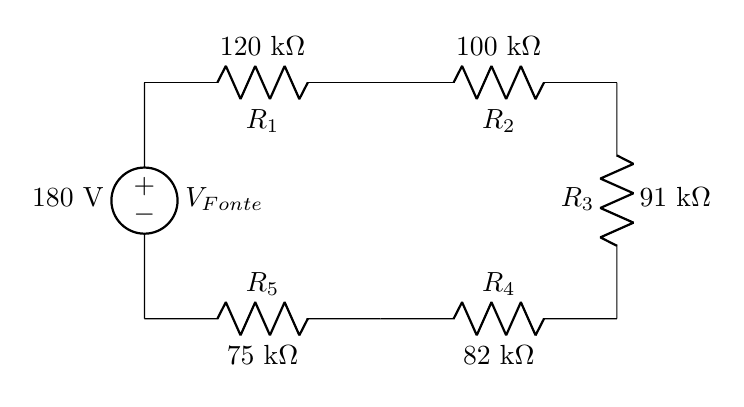
\begin{tikzpicture}[american] %define a tipologia dos componentes do circuito

%O comando \tkzDefPoints define os pontos no plano cartesiano para facilitar o posicionamento dos componentes do circuito. Os pontos são definidos pelas coordenadas (x/y/NomedoPonto)
\tkzDefPoints{
1/4/A,
4/4/B,
7/4/C,
7/1/D,
4/1/E,
1/1/F}

%Do ponto (1,4) ao ponto (4,4) cria um segmento com um resistor (R) no centro. Teste o comando "a" e "l" para incluir o rótulo do resistor, dentro ou fora do elemento. 
%---------------------------------------------------
\draw (A) to [R, a=$R_{1}$, l=$120$ k$\Omega$] (B);
%---------------------------------------------------

%Do ponto (4,4) ao ponto (7,4) cria um segmento com um resistor (R) no centro. Teste o comando "a" e "l" para incluir o rótulo do resistor, dentro ou fora do elemento. 
%---------------------------------------------------
\draw (B) to [R, a=$R_{2}$, l=$100$ k$\Omega$] (C);
%---------------------------------------------------

%Do ponto (7,4) ao ponto (7,1) cria um segmento com um resistor (R) no centro. Teste o comando "a" e "l" para incluir o rótulo do resistor, dentro ou fora do elemento. 
%---------------------------------------------------
\draw (C) to [R, a=$R_{3}$, l=$91$ k$\Omega$] (D);
%---------------------------------------------------

%Do ponto (7,1) ao ponto (4,1) cria um segmento com um resistor (R) no centro. Teste o comando "a" e "l" para incluir o rótulo do resistor, dentro ou fora do elemento. 
%---------------------------------------------------
\draw (D) to [R, a=$R_{4}$, l=$82$ k$\Omega$] (E);
%---------------------------------------------------

%Do ponto (4,1) ao ponto (1,1) cria um segmento com um resistor (R) no centro. Teste o comando "a" e "l" para incluir o rótulo do resistor, dentro ou fora do elemento. 
%---------------------------------------------------
\draw (E) to [R, a=$R_{5}$, l=$75$ k$\Omega$] (F);
%---------------------------------------------------

%Do ponto (1,1) ao ponto (1,4) cria um segmento com uma fonte de tensão (vsource) no centro. Teste o comando "a" e "l" para incluir o rótulo do resistor, dentro ou fora do elemento. 
%---------------------------------------------------
\draw (F) to [vsource, a=$V_{Fonte}$, l=$180$ V, invert] (A);
%---------------------------------------------------

\end{tikzpicture}

\end{document}
